 
\section{Problem 1}
\label{part1}
\begin{enumerate}
\item Write a Python program that extracts 1000 unique links from
Twitter.  You might want to take a look at:

http://thomassileo.com/blog/2013/01/25/using-twitter-rest-api-v1-dot-1-with-python/

\item But there are many other similar resources available on the web.  Note
that only Twitter API 1.1 is currently available; version 1 code will
no longer work.

\item Also note that you need to verify that the final target URI (i.e., the
one that responds with a 200) is unique.  You could have different
shortened URIs for www.cnn.com (t.co, bit.ly, goo.gl, etc.).

\item You might want to use the search feature to find URIs, or you can
pull them from the feed of someone famous (e.g., Tim O'Reilly).

Hold on to this collection -- we'll use it later throughout the semester.
\end{enumerate}

\subsection{Solution}

Extracting 1000 unique links from Twitter was more complex endeavor than expected. 

The following steps were taken in order to get the links 
\begin{enumerate}
\item I did not know where to start,so first i referenced the link provided in the question. This link gave me good idea on how to solve the problem.
\item I got to know that we need to create an app in ``https://apps.twitter.com/'' and then from there i can get my keys in order to hit twitter and get urls.
\item I wrote the code such that i can search for some key words in all the tweets in twitter and get only those tweets which have my key word.
\item This Key word should be given every single time through command prompt and i have queried Subway,Walmart,Trump,McDonalds and Old Dominion to get 1000 urls.
\item I extracted each url using urllib library and saved urls which return status-code as 200 OK.
\item I have had a counter to count my urls and i saved the twitter id,tweet creation date,tweet text and the urls.
\item I preferred to store these files in json format so that it will be well structured and can be easily used in future. 
\item I had gone through a lot of problems with the first program for writing data into json file.
\item There were many other errors coming and i managed to resolve few of those with the help of except block. 
\item Results of my python code are shown below. The output is in the json format. 
\end{enumerate}
\newpage
\subsection{Code Listing}
Here is the python code that is used to collect Thousand URL's from twitter. 


\lstinputlisting[language=Python,breaklines = true,frame=single,caption={Python program for acquiring 1000 unique links for a given keyword}, label=lst:q1-1,captionpos=b,numbers=left,showspaces=false,showstringspaces=false,basicstyle=\footnotesize]{get_1000urls.py}
\newpage
\subsection{Results}
\begin{figure}[ht]    
    \begin{center}
        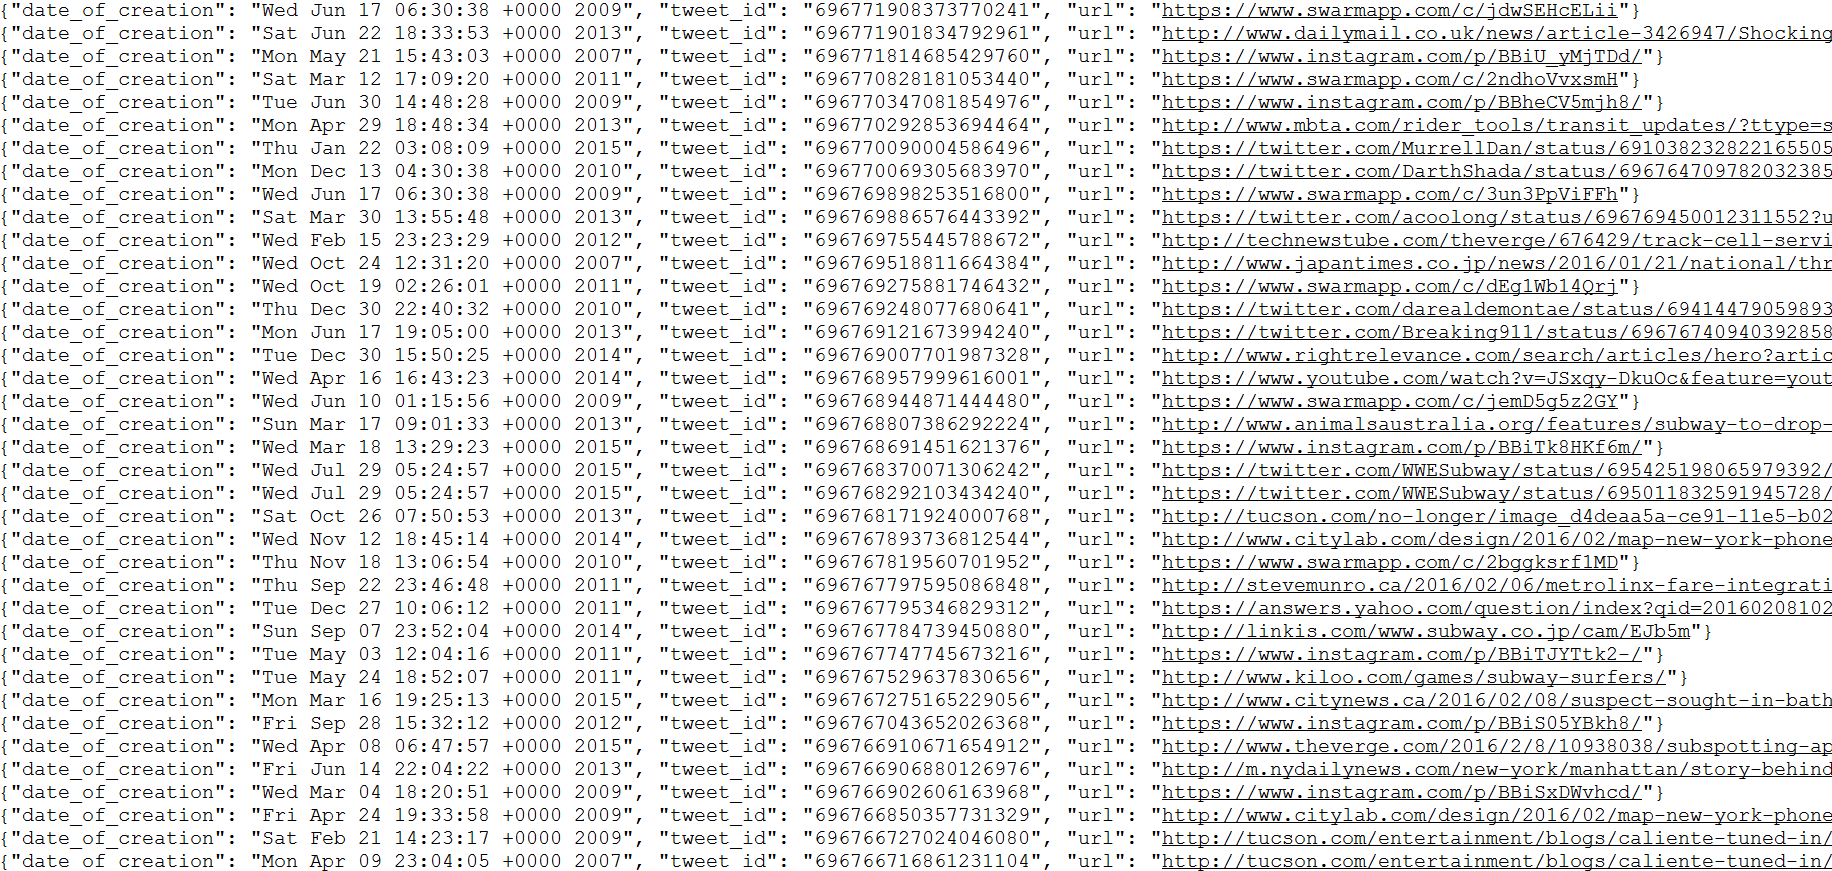
\includegraphics[scale=0.35]{samples_urls.png}
        \caption{Sample Url's}
        \label{Sample Url's}
    \end{center}
\end{figure}

